\documentclass{article} % For LaTeX2e
\usepackage{nips13submit_e,times,graphicx}
\usepackage{hyperref}
\usepackage{url}
%\documentstyle[nips13submit_09,times,art10]{article} % For LaTeX 2.09

\nipsfinalcopy
\title{Learning the Language of the Genome using RNNs}


\author{
Govinda M. Kamath \\
Department of Electrical Engineering\\
Stanford University\\
Stanford, CA 94305 \\
\texttt{gkamath@stanford.edu} \\
\And
Jesse M. Zhang \\
Department of Electrical Engineering \\
Stanford University \\
Stanford, CA 94305 \\
\texttt{jessez@stanford.edu} \\
}

% The \author macro works with any number of authors. There are two commands
% used to separate the names and addresses of multiple authors: \And and \AND.
%
% Using \And between authors leaves it to \LaTeX{} to determine where to break
% the lines. Using \AND forces a linebreak at that point. So, if \LaTeX{}
% puts 3 of 4 authors names on the first line, and the last on the second
% line, try using \AND instead of \And before the third author name.

\newcommand{\fix}{\marginpar{FIX}}
\newcommand{\new}{\marginpar{NEW}}

%\nipsfinalcopy % Uncomment for camera-ready version

\begin{document}


\maketitle

%\begin{abstract}
%The abstract paragraph should be indented 1/2~inch (3~picas) on both left and
%right-hand margins. Use 10~point type, with a vertical spacing of 11~points.
%The word \textbf{Abstract} must be centered, bold, and in point size 12. Two
%line spaces precede the abstract. The abstract must be limited to one
%paragraph.
%\end{abstract}

\section{Introduction}
In recent years, deep recurrent neural networks (RNNs) have allowed researchers to tackle a variety of machine learning problems in the domain of natural language processing. Most of these applications investigate problems such as translation, named entity recognition, and sentiment analysis. Less work has been done with RNNs on what is perhaps the most natural language: the genome. The genome is a sequence of four letters (A, C, G, T). While some deep genomic models (\cite{alipanahi2015predicting},\cite{kelley2015basset},\cite{quang2015danq},\cite{zhou2015predicting}) have emerged in the past two years, none of them process the genome as a natural language. The purpose of this project is to explore how various RNN architectures can be used to learn sequential patterns in various genomes. 

\section{Problem Statement}
Five genome datasets have been prepared for this project:
\begin{enumerate}
	\item A length-30,000 repeating genome where the repeated unit is \texttt{AGCTTGAGGC}
	\item A length-30,000 random genome
	\item The length-4,639,675 genome for \textit{E. coli}
	\item The length-23,264,338 genome for malaria
	\item The length-3,137,161,264 genome for humans 
\end{enumerate}

Depending on computational resources and time, we hope to tackle a variety of questions. First, we will explore an RNN's ability to capture the structure in a given genome. If the ability of an RNN to predict the next character for a real genome is the same as for a random genome, then we have no hope of going further. Once we have empirical evidence that an RNN can capture the non-random structure within a genome, we will explore further classification problems. Decades of wet lab experiments have allowed biologists to classify certain sequences according to their biological function (or the type of cell the sequence is more important for), and these results are available via the ENCODE and Roadmap Epigenomics data releases. We will assess the RNN's ability to classify these sequences after finding a distributed representation for its vocabulary. Defining what this ``vocabulary" is will also be a challenge.

\section{Technical Approach and Models}

Using Google's TensorFlow Python package, we will test a variety of RNN-based neural network architectures including gated recurrent units (GRUs) and long-short-term-memory RNNs (LSTMs). We will experiment with a variety of hyperparameters on multiple datasets in order to assess the robustness of our models. We will measure the ability of a model to fit a given dataset using the average perplexity:

$$
	PP(\mathbf{y},\mathbf{\hat{y}}) = \exp \left\{-\frac{1}{n-1} \sum_{t=1}^{n-1} \sum_{i=1}^{|V|} y_i^{(t)} \log \hat{y}_i^{(t)}\right\}
$$

where $n$ is the number of training samples (roughly the length of our genome), $|V|$ is the size of our vocabulary, $\hat{y}^{(t)}_i$ is the predicted probability of the predicted word at time $t$ being word $i$, and $\mathbf{y}^{(t)}$ is a one-hot vector describing the actual word at time $t$.

We start with a simple model where we predict one character at a time based on previous characters. Once this succeeds, we will play with additional complexity such as bi-directional architecture, multiple layers, and a more complex vocabulary of $n$-grams rather than characters. The first goal of this project is to minimize the perplexity. 

\section{Preliminary Results}

We have successfully ran a simple one directional character-prediction RNN/GRU/LSTM for all the genomes except human. 

Our baselines were the artificial genomes (first two genomes in the list). Any model that does not perform as expected on these two genomes will not be used on other genomes. We want to perform better than the random genome, and the repeating genome serves as an empirical lower bound. For these genomes, we used an LSTM architecture, a dropout keep rate of 1, a batch size of 50, a sequence length of 50, a learning rate of 0.002, and 10 epochs. The achieved perplexity of the random genome was 4.003, just as expected. This is the case when the model always assigns equal probability to each of the 4 possible character A, C, G, T. The achieved perplexity of repeating genome is 1.002, which was also just as expected. Since the sequence repeats without noise, we expect the model to be able to put all the probability mass on a single character.

For the \textit{E. coli} and malaria genomes, we used a dropout keep rate of 1, a batch size of 50, and 1 epoch. We tested the GRU, LSTM, and RNN architectures, learning rates of 0.0001 and 0.0008, sequence lengths of 50, 100, 500, and 1000, and 2 and 3 layers. Because we have not implemented the code on a GPU yet, we had to limit the epoch to 1 in order to test every combination of the above hyperparameters. For both genomes, all combinations of hyperparameters performed about the same, reaching a perplexity of 3.679 for \textit{E. coli} and a perplexity of 2.938 for malaria. All training errors were continuing to decrease after 1 epoch, however, indicating that increasing the epochs will allow for even smaller perplexities (Figures 1 and 2).

The learning rate of 0.0001 performed worse than the learning rate of 0.0008, but this is likely because the former is slower at updating. We will use 0.0008 for future experiments. Both 2 and 3 layers worked about the same, and we will go with a 3 layer network as we suspect a deeper network will benefit more from additional training. Surprisingly, 50 or 100-length sequences perform better than 500 or 1000-length sequences despite the fact that genomes often involve long-range interactions. This may just be a result of not training for enough epochs. We will continue testing different sequence lengths. Finally, both RNNs and GRUs appear to outperform LSTMs. This is surprising to us and we are not sure why RNNs would perform better than LSTMs. We will need to investigate further after training for additional epochs.

\begin{figure*}[!htb]
	\caption{Perplexity as a function of training batch number for multiple combinations of learning rates, number of layers, RNN architectures, and sequence lengths. The \textit{E. coli} genome was used.}
	\centering
	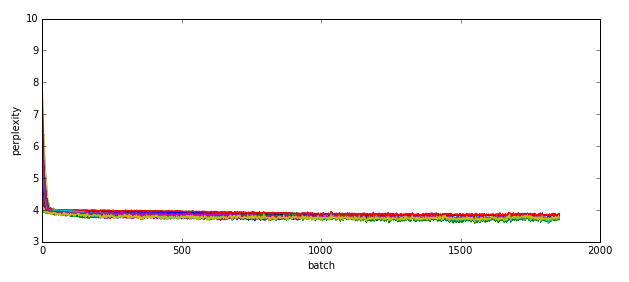
\includegraphics[scale=0.6]{tlecoli}
\end{figure*}
\begin{figure*}[!htb]
	\caption{Perplexity as a function of training batch number for multiple combinations of learning rates, number of layers, RNN architectures, and sequence lengths. The malaria genome was used.}
	\centering
	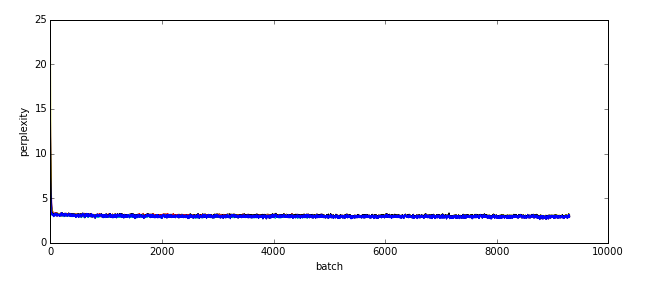
\includegraphics[scale=0.6]{tlmalaria}
\end{figure*}
 
\bibliographystyle{plain}
\bibliography{cs224d}

\end{document}
